%%%%%%%%%%%%%%%%%%%%%%%%%%%%%%%%%%%%%%%%%
% Stylish Article
% LaTeX Template
% Version 2.1 (1/10/15)
%
% This template has been downloaded from:
% http://www.LaTeXTemplates.com
%
% Original author:
% Mathias Legrand (legrand.mathias@gmail.com) 
% With extensive modifications by:
% Vel (vel@latextemplates.com)
% Final ACS by:
% Juan Barbosa
% License:
% CC BY-NC-SA 3.0 (http://creativecommons.org/licenses/by-nc-sa/3.0/)
%
%%%%%%%%%%%%%%%%%%%%%%%%%%%%%%%%%%%%%%%%%
\documentclass[fleqn,11pt]{SelfArx}
%\usepackage[superscript]{cite}
\usepackage{wrapfig}
\usepackage{rotating}
\usepackage{subcaption}
\usepackage[numbers, super]{natbib}
%----------------------------------------------------------------------------------------
%	ARTICLE INFORMATION
%----------------------------------------------------------------------------------------

\JournalInfo{Laboratorio Org\'anica 3, No. 4, 14/10/2017} % Journal information
\Archive{ }

\PaperTitle{Acilación de Friedel-Crafts} %
%\Keywords{Keyword1 --- Keyword2 --- Keyword3} % Keywords - if you don't want any simply remove all the text between the curly brackets
%\newcommand{\keywordname}{Keywords} % Defines the keywords heading name

%----------------------------------------------------------------------------------------
%	ABSTRACT
%----------------------------------------------------------------------------------------

\Abstract{
\begin{wrapfigure}{r}{0.45\textwidth}
	\centering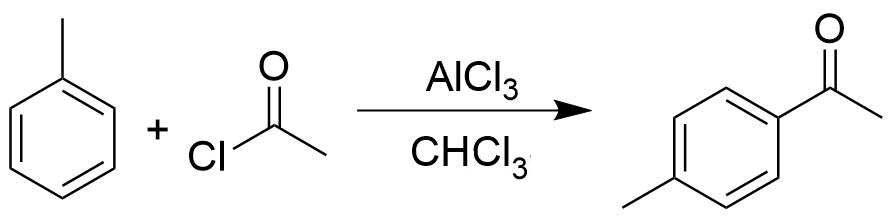
\includegraphics[width=0.95\linewidth]{structures/reaction.png}
\end{wrapfigure}

La preparación de la 4-metilacetofenona se llevó a cabo usando tolueno, cluroro de acetilo, y cloruro de aluminio (III) como ácido de Lewis, en una reacción de acilación de Friedel-Crafts, usando cloroformo como disolvente. La reacción tuvo una duración de 1.5 horas y un rendimiento de 41 \%, sin requerir un tratamiento de purificación. La caracterización del producto se llevó a cabo usando $^1$HRMN y $^{13}$CRMN.
}

%----------------------------------------------------------------------------------------

\begin{document}

\flushbottom % Makes all text pages the same height

\maketitle % Print the title and abstract box

%\tableofcontents % Print the contents section

\thispagestyle{empty} % Removes page numbering from the first page
\renewcommand{\tablename}{Tabla} 


%----------------------------------------------------------------------------------------
%	ARTICLE CONTENTS
%----------------------------------------------------------------------------------------

\section*{Introducci\'on} % The \section*{} command stops section numbering
%------------------------------------------------
Dos reacciones llevan el nombre de los químicos Charles Friedel y James Crafts, ambas reacciones se caracterizan por usar carbocationes como electrófilos capaces de sustituir anillos aromáticos, produciendo un nuevo enlace carbono-carbono. La primera de estas reacciones es la alquilación, en donde un cloruro de alquilo sustituye un hidrógeno de un anillo aromático activado, esto es un anillo con una alta densidad electrónica, en presencia de un ácido de Lewis para formar alquilbecenos. La segunda reacción procede de forma análoga, salvo que se hace uso de un cloruro de acilo para obtener fenil cetonas \cite{Wade2013}. Si bien los cloruros de alquilo y acilo fueron los reactivos inicial propuestos por Friedel y Crafts, existen gran variedad de reacciones que se llevan a cabo con derivados de ácidos, los cuales también pueden general carbocationes \cite{Wade2013}.
\begin{scheme}[h]
	\centering
	\caption{A la izquierda una reacción de alquilación, a la derecha acilación de Friedel-Craft. \ce{X = Cl, Br, I}, \ce{R = alquil, aril} \cite{Wade2013}.}
	\includegraphics[width=1.\linewidth]{structures/FriedelCraft.png}
\end{scheme}
\newpage

Una diferencia importante entre la alquilación y la acilación es la cantidad de ácido de Lewis requerido en la reacción, mientras en la primera se requieren cantidades catalíticas, en la acilación es necesario el uso de un equivalente. A pesar de esto la acilación es considerablemente más usada experimentalmente porque no permite que la reacción se lleve a cabo más de una vez. Esto se debe a que el producto de la reacción es una cetona, donde se tiene unido al anillo un grupo carbonilo, el cual extrae carga, desactivando el mismo. Lo anterior no ocurre con alquilación por lo cual es posible obtener productos polialquilados \cite{Wade2013, sartori_maggi_2010}.
\begin{scheme}
	\centering
	\caption{Obtención de la \textit{ortho}-hidroxiacetofenona usando una reacción de Friedel-Crafts con \'acido acético como generador del carbocatión \cite{davenport1986process}.}
	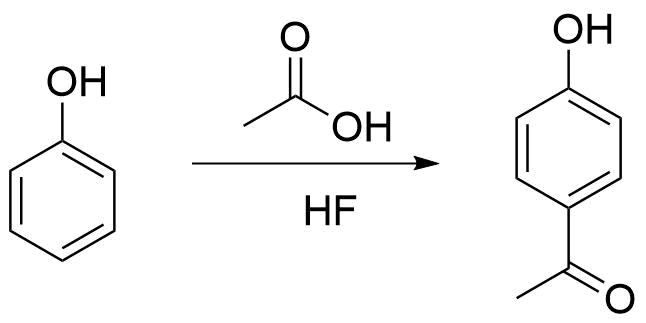
\includegraphics[width=0.6\linewidth]{structures/hidroxiacetofenona.png}
\end{scheme}

Por estas razones la acilación de Friedel-Crafts se considera un pilar fundamental en la química orgánica sintética, existen al menos 20 mil referencias que involucren esta reacción \cite{sartori_maggi_2010}. Las cetonas aromáticas obtenidas constituyen importantes intermediarios en productos farmaceúticos, y agroquímicos, entre otros. Por ejemplo la \textit{ortho}-hidroxiacetofenona constituye un importante precursor en la síntesis de la 4-hidroxicumarina, el cual se obtiene por la reacción de fenol con ácido acetico o anhídrido acético \cite{sartori_maggi_2010, davenport1986process}. Siendo la 4-hidroxicumarina una molécula de especial importancia farmacéutica esto debido a su actividad antitumoral y contra el VIH \cite{Mahajan2009, Maresca2010}.

El mayor uso de la 4-metilacetofenona es como aditivo alimenticio, especificamente como agente saborizante, según la clasificación de la Comisión Europea para los agentes de mejoramiento de la comida\cite{Demyttenaere2012}.

\section{Resultados y Discusi\'on}
La molécula preparada en el laboratorio cuenta con un plano de simetría lo cual implica que existen únicamente 4 señales de hidrógeno de los 10 que se encuentran en la molécula. De igual manera para los carbonos se observan 7 señales distintas de los 9 carbonos que se tienen en la muestra. En el caso de los hidrógenos se observan las siguientes señales (\autoref{HRMN}): $\delta$ 2.41 \textbf{(a)}, 2.59 \textbf{(b)}, 7.26 \textbf{(c)} y 7.86 \textbf{(d)}. Estos desplazamientos corresponden con los reportados en la literatura \cite{Liu2010}. Tanto las señales \textbf{(a)} como \textbf{(b)} corresponden con los grupos metilo del anillo y la cetona correspondientemente, por lo cual integran para 3 hidrógenos cada uno y señales singletes. El desplazamiento químico es mayor para el caso del metilo de la cetona dado que el grupo carbonilo extrae mayor cantidad de carga que el anillo. En el caso de las señales de carbono estos grupos también corresponden con las señales \textbf{(a)} $\delta$ 21.48 y \textbf{(b)} $\delta$ 26.58, siguiendo la misma tendencia en el desplazamiento que los protones.
\begin{scheme}[h]
	\centering
	\caption{Asignación de señales de RMN. En azul se muestran las señales para protones y en rojo para carbonos.}
	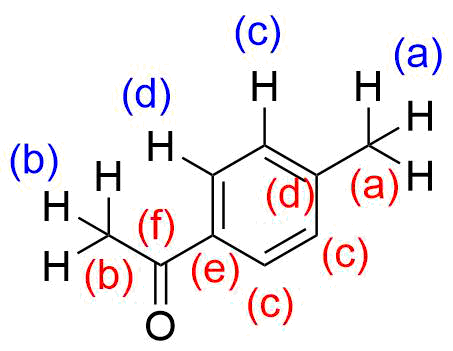
\includegraphics[width=0.45\linewidth]{structures/asignacion.png}
\end{scheme}

Posteriormente a campo bajo se encuentran las señales aromáticas que en el caso del carbono las primeras corresponden con los átomos \textit{ortho} a ambos grupos, las cuales se solapan y se observan como una única señal \textbf{(c)} $\delta$ 128.83. En el caso de los hidrógenos, existen dos efectos a tener en cuenta por un lado el grupo metilo (activante) agrega carga sobre el hidrógeno \textbf{(d)}, de la misma forma que la cetona protege la posición meta, este efecto implicaría que la señal \textbf{(d)} aparece a campo más alto, sin embargo el enlace $\pi$ del carbonilo puede entrar en resonancia con el anillo agregando densidad una densidad de carga superior al hidrógeno \textbf{(c)}, siendo este último efecto el que prima en la molécula. Es por esta misma razón que en carbonos la señal \textbf{(d)} se encuentra a campo más alto que la señal \textbf{(e)}, $\delta$ 134.76, 143.87 correspondientemente. Finalmente el carbono más desprotegido corresponde con el carbono carbonílico que aparece en $\delta$ 197.84 \textbf{(f)}.

El experimento DEPT-135 confirma la identidad de los carbonos dado que las señales \textbf{(d)}, \textbf{(e)}, y \textbf{(f)} no se observan al ser carbonos cuaternarios. El resto de señales observadas corresponden a carbonos primarios y terciarios, por lo cual se observan con intensidades positivas.

Los resultados obtenidos por resonancia magnética nuclear permiten determinar que el producto se encuentra puro, por lo cual el porcentaje de recuperación corresponde con el rendimiento de la reacción, el cual es de 41 \%. Además que la existencia de dobletes para las señales \textbf{(c)} y \textbf{(d)} para los hidrógenos confirma la selectividad de la reacción hacia el producto \textit{(para)}. Siendo esto un hecho explicable desde el mecanismo de reacción y la energía de las moléculas.

A nivel experimental la reacción tiene lugar en dos etapas, la primera es la formación del carbocatión y la segunda la sustitución electrofílica aromática. El mecanismo así mismo se puede dividir en estas dos etapas. El primer paso es el ataque del cloro del cloruro de acilo al ácido de Lewis \textbf{(a)}, el cual forma un complejo ionico que posteriormente se descompone para dar lugar a la formación del carbocatión, el cual se encuentra estabilizado por la resonancia del enlace $\pi$ del carbonilo \textbf{(c)}.
\begin{scheme}[h]
	\centering
	\caption{Formación del carbocatión en la primera parte de la reacción \cite{Wade2013}.}
	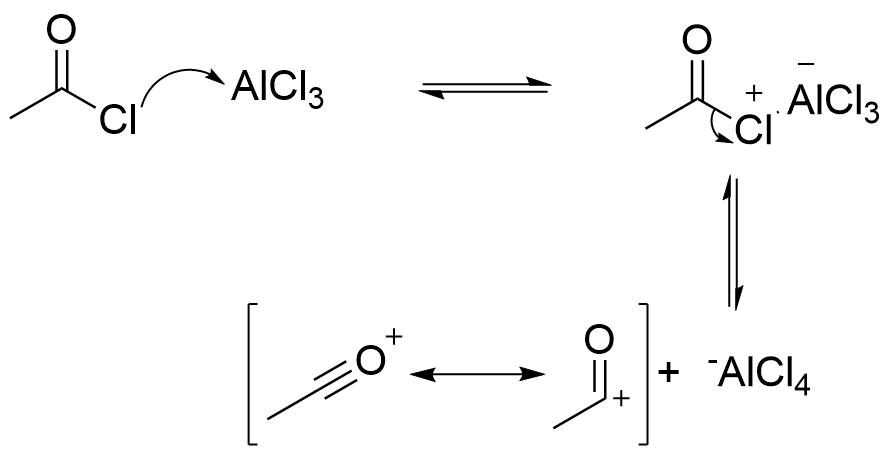
\includegraphics[width=0.9\linewidth]{structures/mechanism1.png}
\end{scheme}

\begin{scheme*}[h]
	\centering
	\caption{Complejo sigma. Las estructuras en azul son particularmente estables por la densidad de carga del metilo, además de ser carbocationes terciarios.}
	\includegraphics[width=0.7\linewidth]{structures/SigmaComplex.png}
	\label{sch: sigma}
\end{scheme*}

Resulta importante que el carbocatión se encuentre aislado del aire, el cual al contener vapor de agua fácilmente puede hidrolizar al catión, degradando el reactivo límite, limitando el rendimiento, lo cual no se descarta haya ocurrido en el caso del presente documento.
\newpage

\begin{figure*}[ht]
	\centering
	\begin{tabular}{ccc}
		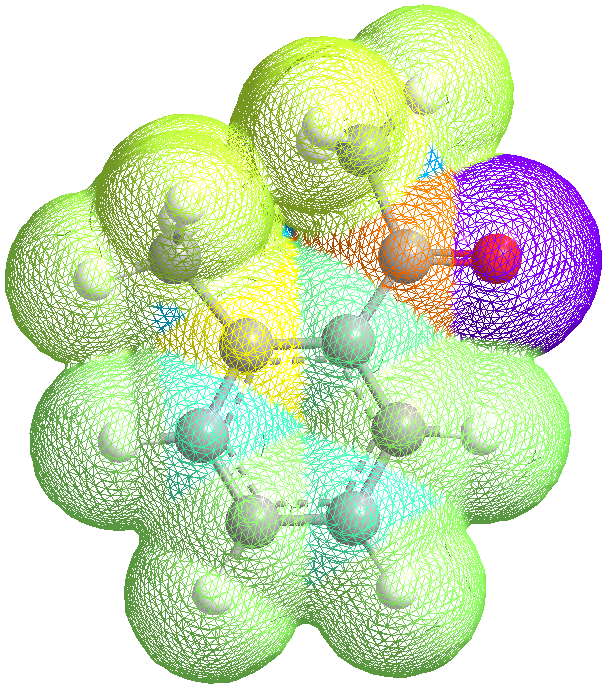
\includegraphics[width=0.3\linewidth]{structures/ortho.png} & 
		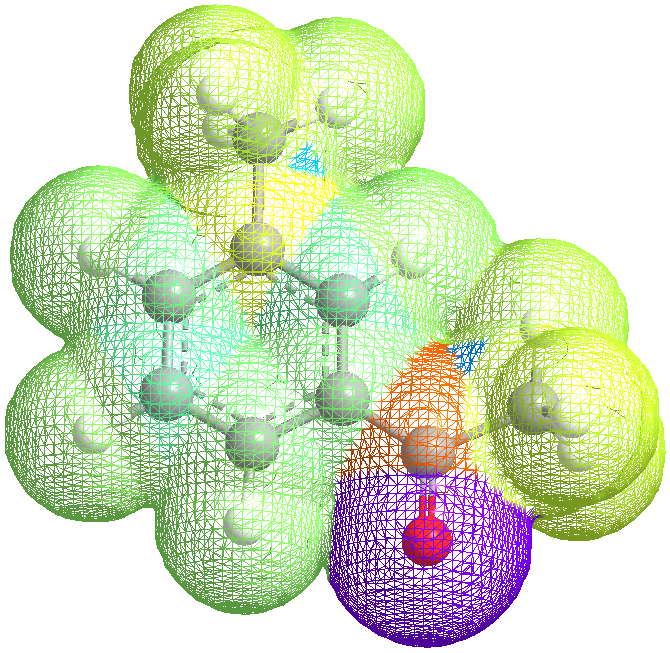
\includegraphics[width=0.3\linewidth]{structures/meta.png} &
		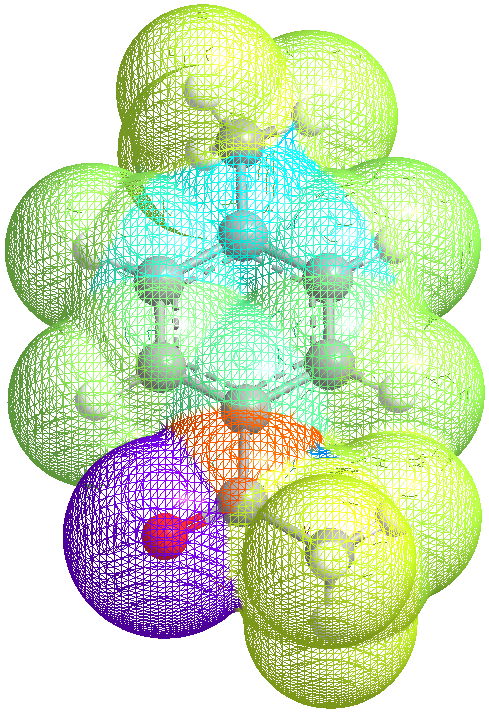
\includegraphics[width=0.25\linewidth]{structures/para.png}
	\end{tabular}
	
	\caption{Moléculas aciladas en las posiciones \textit{ortho}, \textit{meta}, y \textit{para} correspondientemente. Las energias de MM2 (\textit{Mining-Minima}) son: 14.49 kcal/mol, 8.99 kcal/mol, 8.83 kcal/mol.}
	\label{fig: energy}
\end{figure*}

El ataque nucleofílico del anillo puede tener lugar en tres posiciones distintas: \textit{ortho} \textbf{(d1)}, \textit{meta} \textbf{(d2)}, \textit{para} \textbf{(d3)}. Para el caso de las posiciones \textit{ortho} y \textit{para} existe una estructura resonante adicional a la mostrada en el \autoref{sch: sigma}, en donde en las estructuras azules un par electrónico del metilo baja sustituye la carga positiva del anillo y se obtiene un carbocatión primario, sin embargo al ser un catión primario no es una estructura que contribuya realmente en la estabilización del intermediario. Se dice que las estructuras del \autoref{sch: sigma} que se encuentran en azul son más estables porque al ser el metilo un grupo activador pueden estabilizar parte de la densidad de carga positiva además de formar un carbocatión terciario \cite{Wade2013}. Lo anterior reduce la posibilidad de formación de los tres productos de acilación a dos, los de posición \textit{ortho} y \textit{para}.
\begin{scheme}[h]
	\centering
	\caption{Pérdida de un protón y regeneración de la aromaticidad. Obtención de la metilacetofenona libre.}
	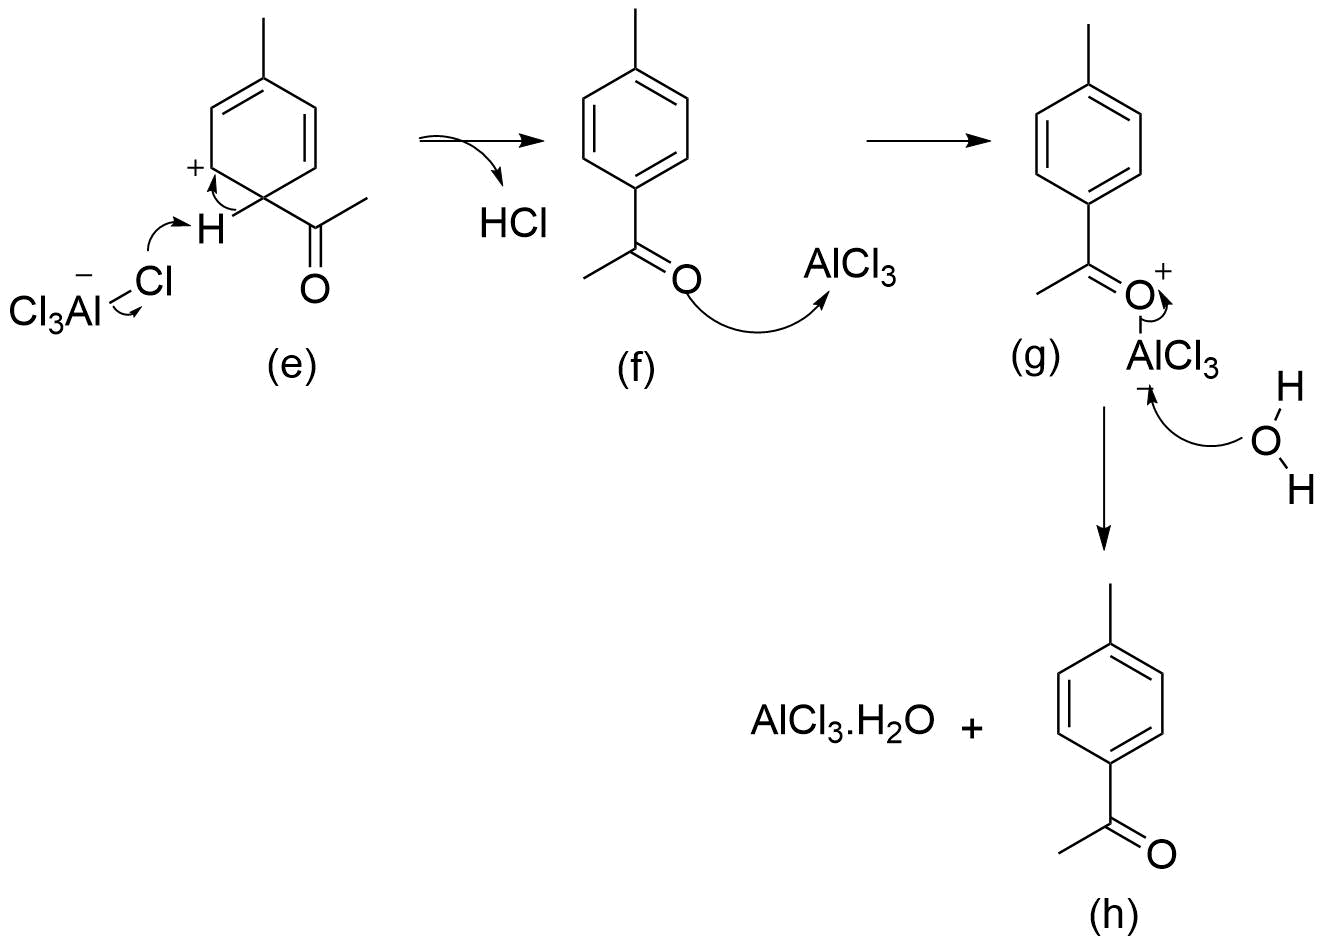
\includegraphics[width=\linewidth]{structures/mechanism2.png}
\end{scheme}

El cloro de un anión de cloruro de aluminio ataca al protón que se encuentra en la posición de sustitución el cual al salir regenera la aromaticidad del ciclo \textbf{(e)}, posteriormente el oxígeno de la acetofenona se coordina con el cloruro de aluminio (III) \textbf{(f)}. Para realizar el \textit{quench} de la reacción se usa un exceso de agua el cual libera la acetofenona y genera el hidrato del cloruro \textbf{(g)}.

Estos últimos pasos son análogos para la sustitución en \textit{ortho} y \textit{para}, sin embargo el impedimento estérico es considerablemente menor para el caso del compuesto \textit{para}, el cual se cuantifica con los resultados de una simulación de minimización de energía usando el método de \textit{Mining-Minima} \cite{Huang2012}. Los resultados se observan en la siendo la \autoref{fig: energy}, donde para la molécula sustituída en posición \textit{para} la energía obtenida corresponde con 8.83 kcal/mol. Esta energía corresponde con cerca del 61 \% de la energía del compuesto \textit{ortho}. Lo anterior explica cuantitativamente el efecto del impedimento estérico en la posición de la sustitución.

Finalmente y con el objetivo de mejorar el rendimiento de la reacción se propone 
\newpage

\section{Conclusiones}

\section{Secci\'on experimental}
En un balón de reacción sobre un baño de hielo son adicionados 2.5 mL (23.04 mmol) de cloroformo y 0.410 mL (3.86 mmol) de tolueno, ambos secos con tamiz molecular. A esta solución se adiciona gota a gota una mezcla con 0.480 g de cloruro de aluminio (3.60 mmol) y 0.267 g de cloruro de acetilo (3.40 mmol), limitando la exposición al aire. La reacción tiene lugar a temperatura ambiente por 1 hora y 30 minutos. Posteriormente se realiza una extracción líquido-líquido con diclorometano. La fase orgánica se lava con una solución saturada de bicarbonato. Finalmente la solución se seca usando sulfato de sodio y el disolvente se evapora a presión reducida.

\paragraph{4-metilacetofenona:}
$^1$H NMR (400 MHz, \ce{CDCl3}) $\delta$ 7.86 (d, J = 8.2 Hz, 2H), 7.26 (d, J = 7.9 Hz, 2H), 2.59 (s, 3H), 2.41 (s, 3H).

$^{13}$C NMR (101 MHz, \ce{CDCl3}) $\delta$ 197.84 (s), 143.87 (s), 134.76 (s), 128.83 (s), 26.58 (s), 21.48 (s).

%----------------------------------------------------------------------------------------
%	REFERENCE LIST
%----------------------------------------------------------------------------------------
%\newpage
\phantomsection
\bibliography{informe}
\bibliographystyle{achemso}

%----------------------------------------------------------------------------------------
\onecolumn
\section{Informaci\'on suplementaria}\label{sec: complementaria}

\rotatebox{90}
{
	\begin{minipage}{0.9\textheight}
		\centering
		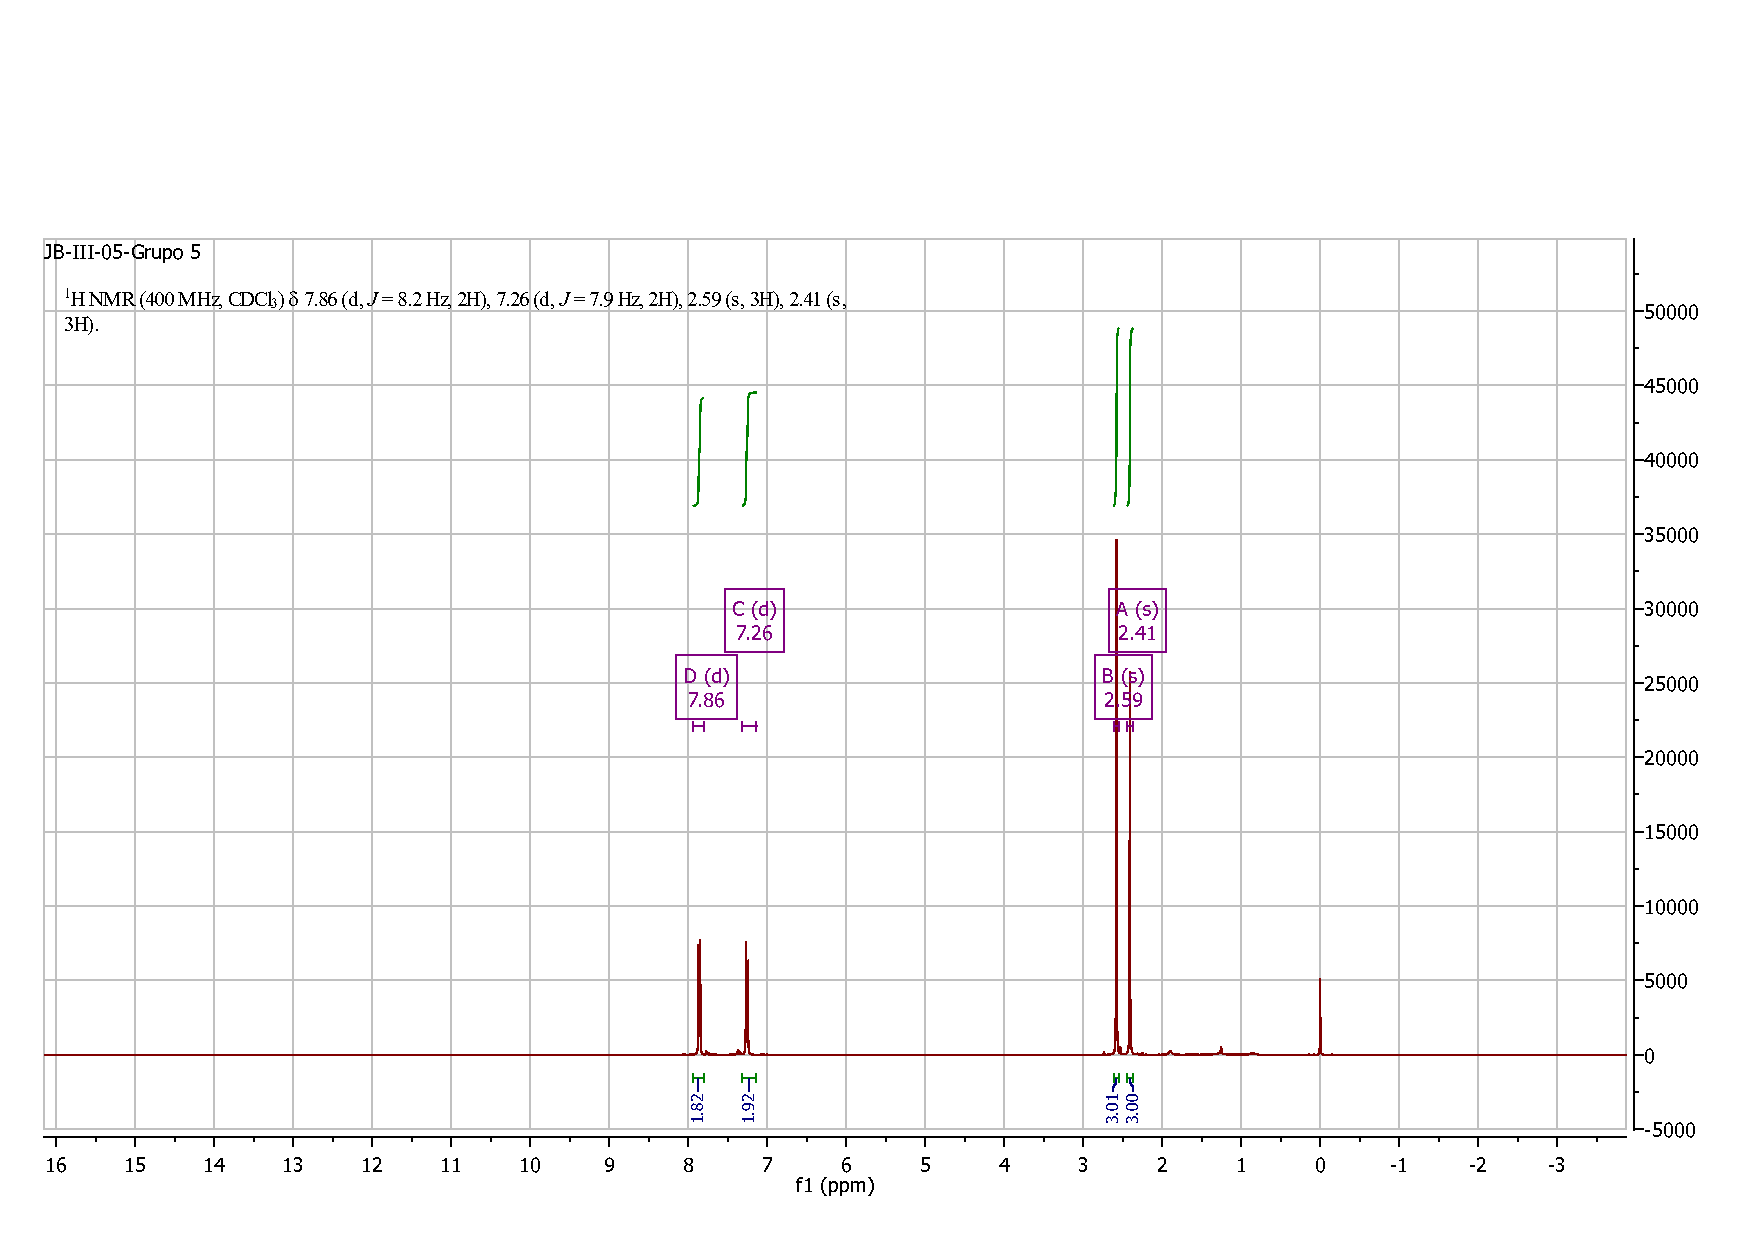
\includegraphics[height=0.7\textheight]{RMN/HRMN.pdf}
		\captionof{figure}{$^1$HRMN del producto.}
		\label{HRMN}
	\end{minipage}
}

\rotatebox{90}
{
	\begin{minipage}{\textheight}
		\centering
		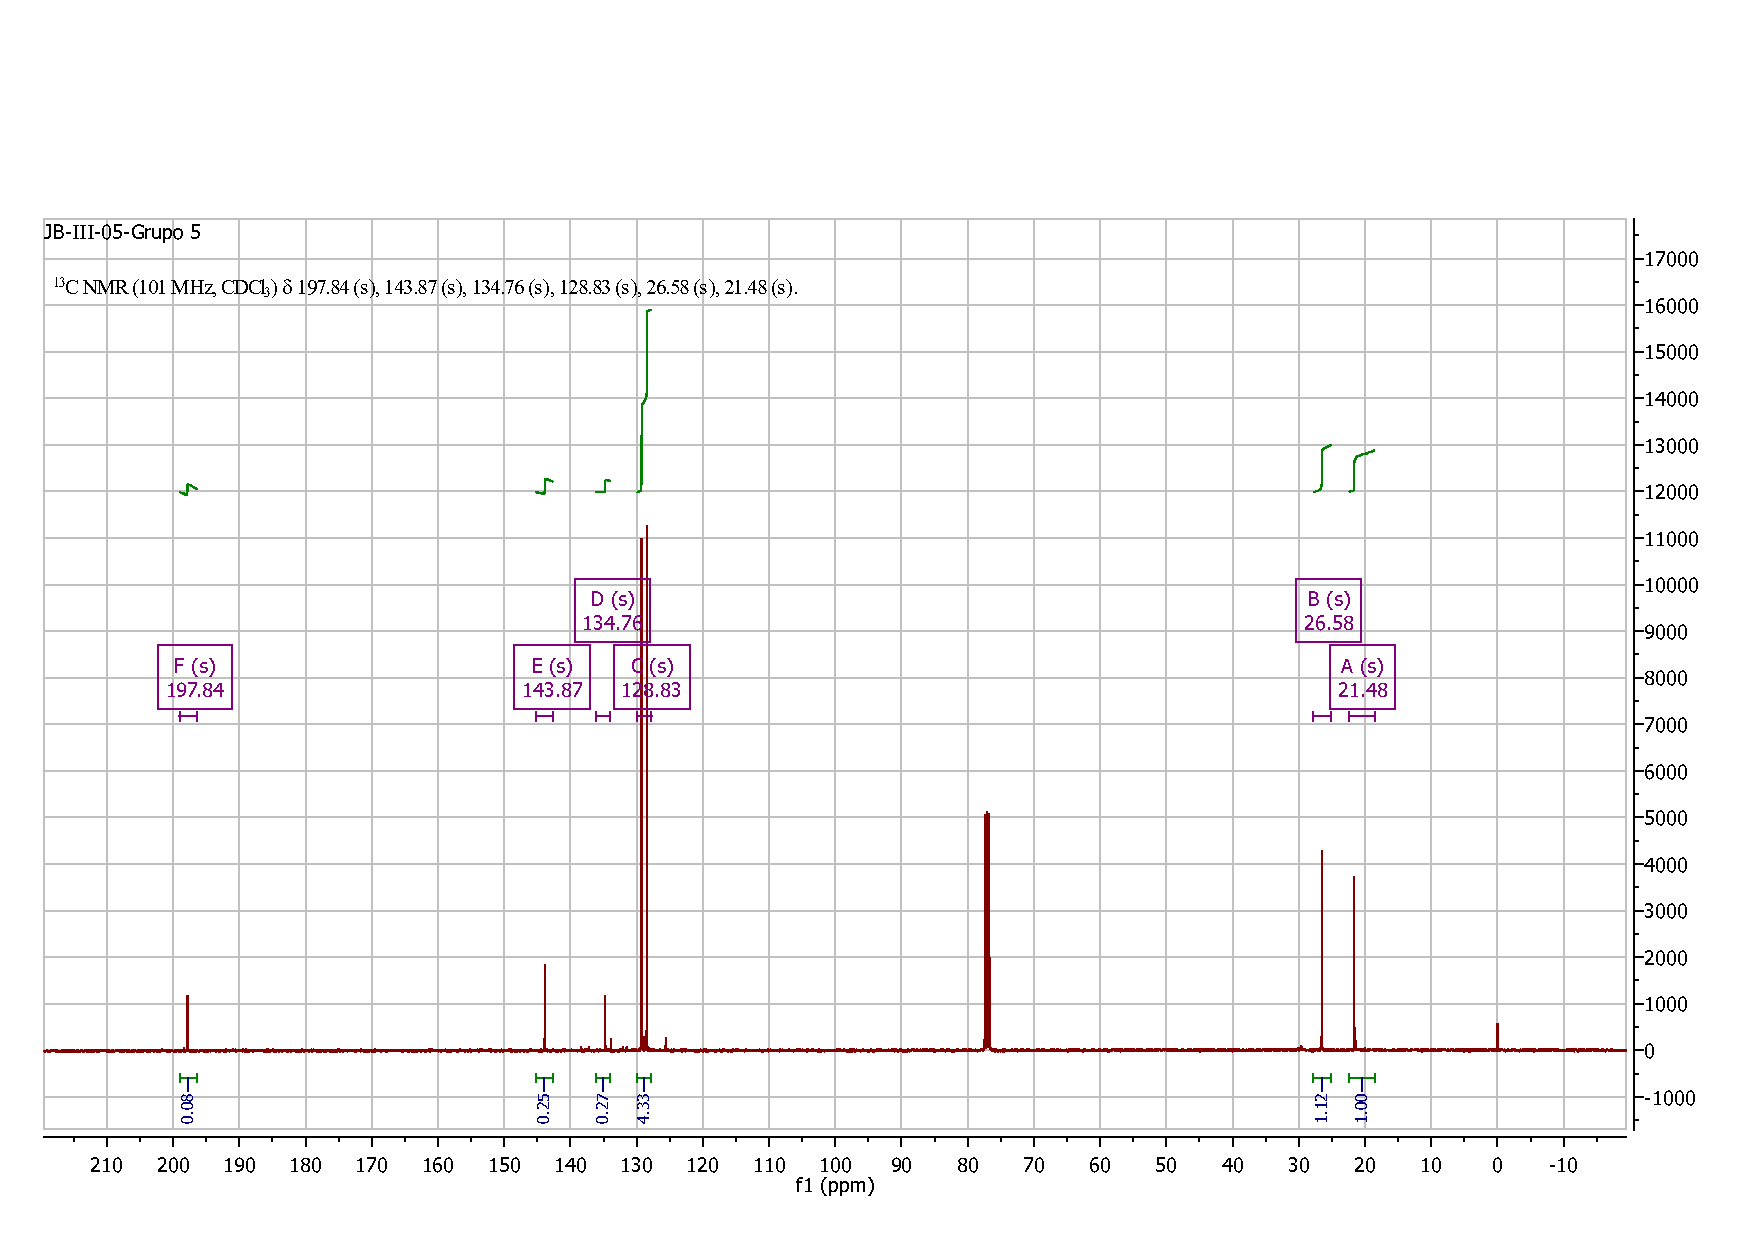
\includegraphics[height=0.7\textheight]{RMN/CRMN.pdf}
		\captionof{figure}{$^{13}$CRMN del producto.}
		\label{CRMN}
	\end{minipage}
}

\rotatebox{90}
{
	\begin{minipage}{\textheight}
		\centering
		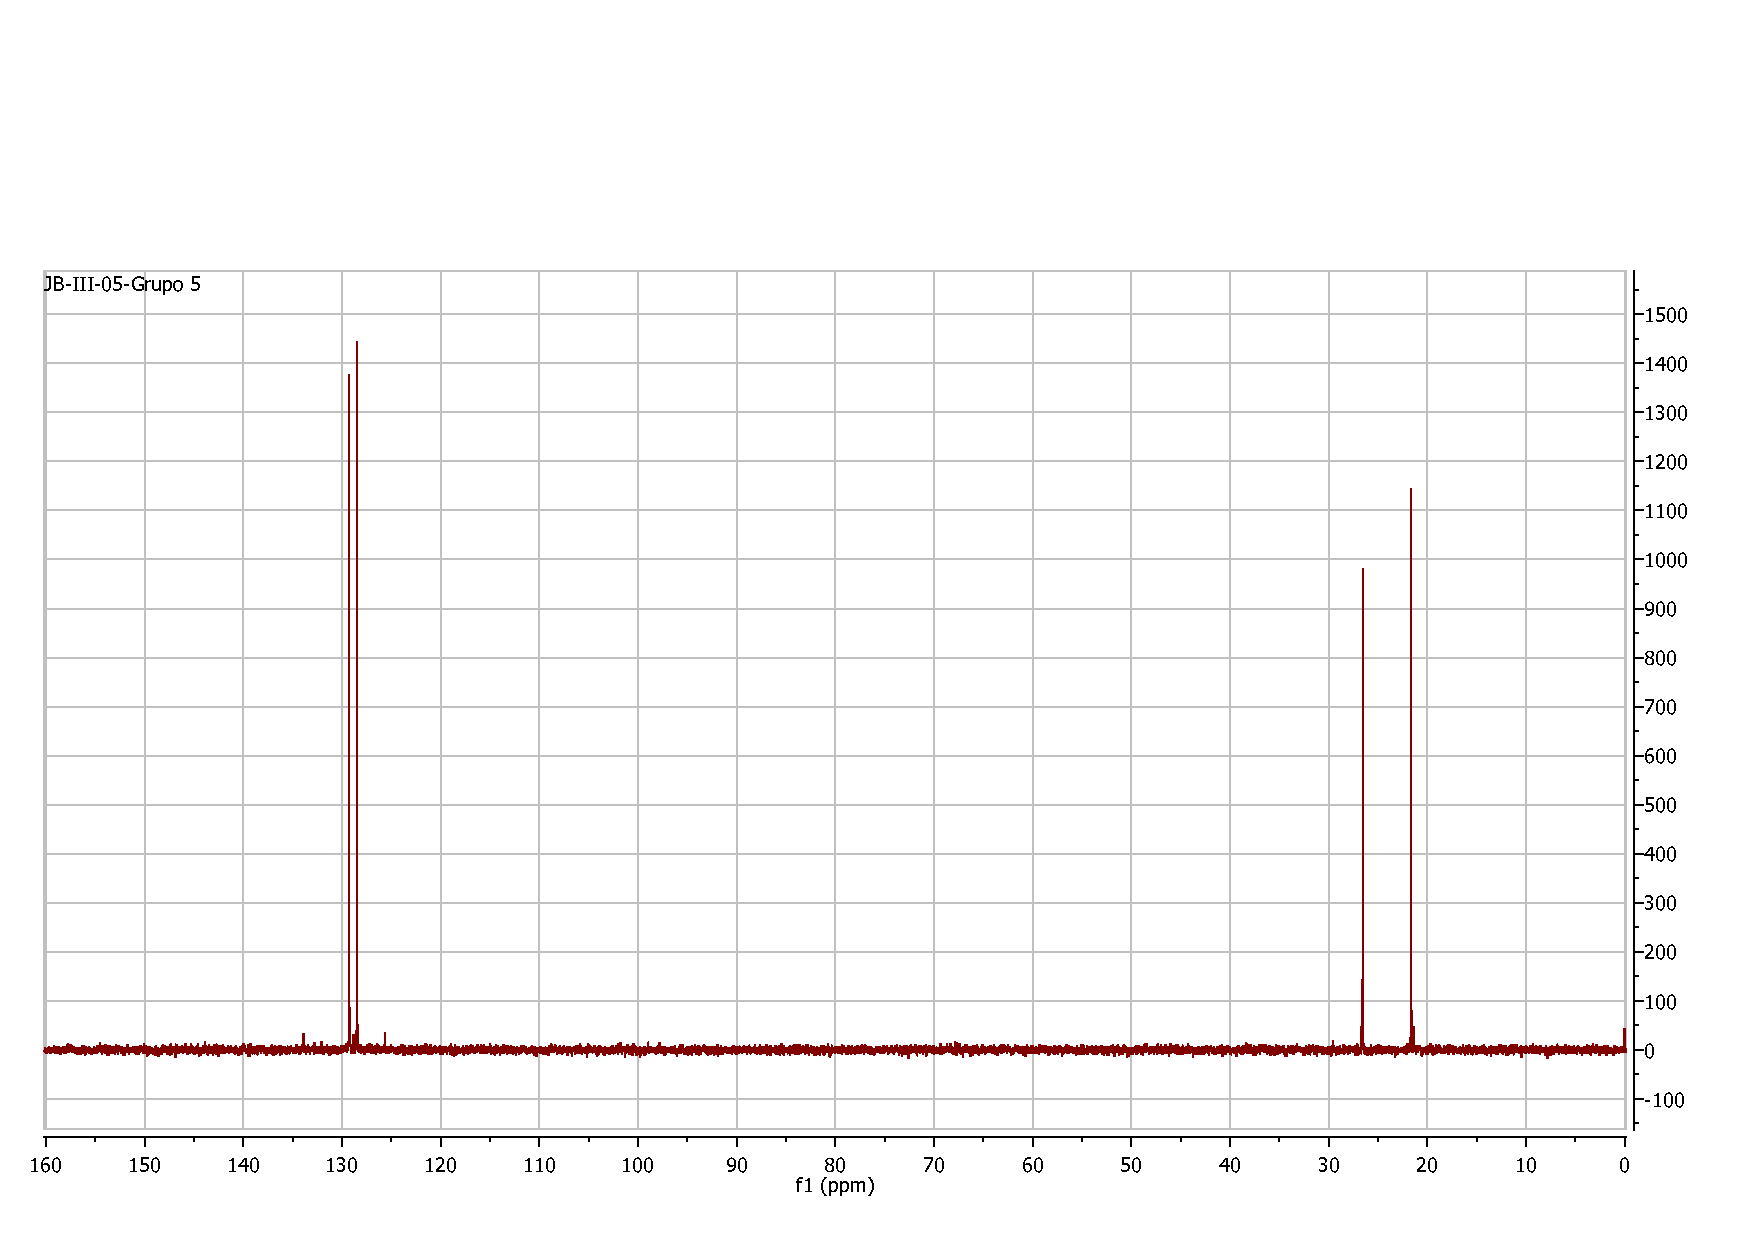
\includegraphics[height=0.7\textheight]{RMN/DEPTRMN.pdf}
		\captionof{figure}{Experimento DEPT-135 del producto.}
		\label{DEPT}
	\end{minipage}
}
\end{document}